% !TeX spellcheck = de_DE
\documentclass[
			   fontsize=11pt,
               paper=a4,
               bibliography=totoc,
               idxtotoc,
               headsepline,
               footsepline,
               footinclude=false,
               BCOR=12mm,
               DIV=13,
               openany,   % using this removes blank pages around part / chapter starts.
%               oneside    % include this if you have to print only one page per sheet of paper.
               ]
               {scrbook}

%%% SETTINGS

% no word wrapping
%\righthyphenmin=62
%\lefthyphenmin=62
% fewer hyphens
\usepackage{microtype}

% german symbols
\usepackage[utf8]{inputenc}

% strikethrough by \sout
\usepackage[normalem]{ulem}

% insert graphics
\usepackage{graphicx}
% more flexible figures e.g. graphics with captions beside them
\usepackage{floatrow}
% more flexible captions.
% Use \captionsetup{options} to configure,
% use it in an environment for local setup
\usepackage{caption}
% subfigures (see template):
\usepackage{subcaption}

% more control of enumerations and itemizations
\usepackage{enumitem}
% less space between items
\setlist[itemize]{itemsep=0cm}
\setlist[enumerate]{itemsep=0cm}
% more customizeable tables (e.g. multiple lines per cell)
\usepackage{tabularx}
% fix for vertical centering
\usepackage{ragged2e}
\renewcommand\tabularxcolumn[1]{>{\Centering}m{#1}}
% column types with multiple lines and formatting
\usepackage{array}
\newcolumntype{C}{>{\centering\arraybackslash}X}
\newcolumntype{R}{>{\raggedleft\arraybackslash}X}
\newcolumntype{L}{>{\raggedright\arraybackslash}X}
% merge multiple rows \multirow{2}{*}{bla} & \\ &
\usepackage{multirow}
% activate for tables with page breaking
%\usepackage{ltablex}
% fix for table movement and itemizations
%\keepXColumns

% fix for dynamics spaces after custom commands
\usepackage{xspace}

% tabbing: use with \tab
\usepackage{tabto}
\TabPositions{4cm}

%% fancy math
% propper matrices, underbrace text
%\usepackage{amsmath}
\usepackage{mathtools}
% special symbols e.g. squares
\usepackage{amssymb}

% code coloring
\usepackage[dvipsnames]{xcolor} % must be declared before pgfplots, tikz or pstricks package, otherwise it will not work.

%% plotting
\usepackage{pgfplots}
\usepgfplotslibrary{fillbetween}

%%Settings for code
% code placement right there
\usepackage{float}
% code listing
\usepackage{listings}

% flexible multi column style
\usepackage{multicol}

% graphs
\usepackage{tikz}
\usetikzlibrary{shapes.geometric, arrows}
% define some elements
\tikzstyle{box} = [rectangle, rounded corners, minimum width=3cm, minimum height=1cm,text centered, draw=black, fill=black!5]
\tikzstyle{arrow} = [thick,->,>=stealth]
\usepackage{varwidth}

% Some code highlighting styles you can use with lstlistings
% C++ code style similar to default eclipse
\lstdefinestyle{eclipse-cpp} {
    captionpos=b,
    language=C++,
    otherkeywords={final},
    basicstyle=\footnotesize,
    numbers=left,
    numberstyle=\small,
    showstringspaces=false,
    tabsize=2,
    frame=single,
    breaklines=true,
    keywordstyle=\bfseries\color[RGB]{127,0,85},
    identifierstyle=\color[RGB]{0,0,192},
    stringstyle=\color[RGB]{42,0,255},
    commentstyle=\color[RGB]{63,127,95},
    aboveskip=1em,
    belowskip=1em,
}

\lstdefinestyle{standard} {
	basicstyle=\footnotesize\ttfamily, 
	captionpos=b,
	numbers=left,
	numberstyle=\small,
	showstringspaces=false,
	tabsize=2,
	frame=single,
	breaklines=true,
	aboveskip=1em,
	belowskip=1em,
}

% If no highlighting is intended
\lstdefinestyle{plain}{
	basicstyle=\ttfamily\footnotesize,
	aboveskip=1em,
	belowskip=1em,
}

%
\lstdefinelanguage{Kotlin}{
	comment=[l]{//},
	commentstyle={\color{gray}\ttfamily},
	emph={filter, first, firstOrNull, forEach, lazy, map, mapNotNull, println},
	emphstyle={\color{OrangeRed}},
	identifierstyle=\color{black},
	keywords={!in, !is, abstract, actual, annotation, as, as?, break, by, catch, class, companion, const, constructor, continue, crossinline, data, delegate, do, dynamic, else, enum, expect, external, false, field, file, final, finally, for, fun, get, if, import, in, infix, init, inline, inner, interface, internal, is, lateinit, noinline, null, object, open, operator, out, override, package, param, private, property, protected, public, receiveris, reified, return, return@, sealed, set, setparam, super, suspend, tailrec, this, throw, true, try, typealias, typeof, val, var, vararg, when, where, while},
	keywordstyle={\color{NavyBlue}\bfseries},
	morecomment=[s]{/*}{*/},
	morestring=[b]",
	morestring=[s]{"""*}{*"""},
	ndkeywords={@Deprecated, @JvmField, @JvmName, @JvmOverloads, @JvmStatic, @JvmSynthetic, Array, Byte, Double, Float, Int, Integer, Iterable, Long, Runnable, Short, String},
	ndkeywordstyle={\color{BurntOrange}\bfseries},
	sensitive=true,
	stringstyle={\color{ForestGreen}\ttfamily},
}

% fancy algorithms (see template)
\usepackage[ruled, vlined, linesnumbered]{algorithm2e}
\DontPrintSemicolon
\SetKw{KwBy}{by}
\SetKw{KwAnd}{and}

% clickable links and clickable table of content <3
% Options: links with linebreaks
\PassOptionsToPackage{hyphens}{url}
\usepackage[bookmarks=false]{hyperref}
\hypersetup{
    colorlinks,
    citecolor=black,
    filecolor=black,
    linkcolor=black,
    urlcolor=black
}
% Alterations to labels used by \autoref{}: Capitalize everyything
\def\chapterautorefname{Chapter}
\def\sectionautorefname{Section}
\def\subsectionautorefname{Subsection}
\def\algorithmautorefname{Algorithm}
\def\subfigureautorefname{Figure}
% for custon stuff like use:
% \hyperref[custom:foo]{Custom~\ref*{custom:foo}}

% -------------------------------------------------------------------------------
% ------------------------- Bibliography Customisation ------------------------
% -------------------------------------------------------------------------------

% replace \makebibliography with this package to enable nice formatting for citing web pages
\usepackage[%
backend=bibtex				% biber or bibtex
,style=numeric-comp		% numerical-compressed TODO: Check if plain is fine as style (was 'alpha' before I changed it)
,sortcites=true				  % sorts citations if multiple entry keys are passed to a citation command
,isbn=true
,url=true
,doi=true
%,natbib=true         % if you need natbib functions
]{biblatex}
\addbibresource{literature.bib}  % better than \bibliography
\usepackage{lipsum} % for filling pages with stuff

% -------------------------------------------------------------------------------
% -------------------------- Glosssary Customisation --------------------------
% -------------------------------------------------------------------------------
% For some reason this did not work when located in settings.tex
% Any links in resulting glossary will not be "clickable" unless you load the glossaries package after the hyperref package.

\usepackage{xparse}
\usepackage[acronym,toc]{glossaries}

\DeclareDocumentCommand{\newdualentry}{O{}D<>{}m m m m m } {
	\newglossaryentry{gls-#3}{
		name={#5},
		text={#5\glsadd{gls-#3}},
		description={#6},
		plural={#7},
		#1
	}
	\newacronym[see={[Glossary:]{gls-#3}},#2]{#3}{#4}{#5\glsadd{gls-#3}}
}

% use the \newdualentry command like this:
% \newdualentry{OWD}    																			% label
% 	{OWD}		            																				 % abbreviation
% 	{One-Way Delay} 	   																				% long form
% 	{The time a packet uses through a network from one host to another}	  % description
%   {OWDs}																							   % abbreviation in plural

\makeglossaries
% -------------------------------------------------------------------------------
% ---------------------- Acronyms and Glossary Definition ---------------------
% -------------------------------------------------------------------------------

\newacronym{nnapi}{NNAPI}{Neural Networks API}

\newacronym{cv}{CV}{Computer Vision}

\newacronym{cnn}{CNN}{Convolutional Neural Network}

\newacronym{resnet}{ResNet}{Residual Neural Network}

\newacronym{relu}{ReLU}{Rectified Linear Unit}

\newacronym{ml}{ML}{Machine Learning}

\newacronym{nn}{NN}{Neural Network}

\newacronym{ann}{ANN}{Artificial Neural Network}
	
	
\newdualentry{api} %oxford dictionary
	{API}
	{application programming interface}
	{set of functions and procedures allowing the creation of applications that access the features or data of an operating system, application, or other service}
	{APIs}

\newglossaryentry{dl} %oxford dictionary
{
	name={deep learning},
	description={type of machine learning based on artificial neural networks in which multiple layers of processing are used to extract progressively higher level features from data}
	% is a branch of machine learning utilising artificial neural networks for information processing. The extensive internal structure of these networks is characterised by numerous intermediate ("hidden") layers between the input layer and the output layer
}

\newglossaryentry{diff_privacy} %https://oconnell.fas.harvard.edu/files/salil/files/differential_privacy_primer_nontechnical_audience.pdf
{
	name={differential privacy},
	description={protects an individual’s information essentially as if her information were not used in the analysis at all, in the sense that the outcome of a differentially private algorithm is approximately the same whether the individual’s information was used or not}
}

% -------------------------------------------------------------------------------
% --------------------------------- Thesis Info ---------------------------------
% -------------------------------------------------------------------------------

% set title, authors and stuff for the cover
% docytype needs xspace because it is used within text.
\def\doctype{Bachelor's Thesis\xspace}

\def\studyProgram{Informatics}
\def\title{Implementing a mobile app for object detection}

\def\titleGer{Entwicklung einer mobilen App zur Objekterkennung}
\def\author{David Drews}
% Prof
\def\supervisor{Univ.-Prof. Dr. Hans-Joachim Bungartz}
% PhD Candidate
\def\advisor{Severin Reiz, M.Sc.}
\def\date{15th of August 2021}

\begin{document}
\frontmatter
% -------------------------------------------------------------------------------
% ---------------------------------- COVERPAGE ------------------------------
% -------------------------------------------------------------------------------

% correct BCOR - undo at the end !!!
\def\bcorcor{0.15cm}
\addtolength{\hoffset}{\bcorcor}
\thispagestyle{empty}
\vspace{4cm}
\begin{center}
    \includegraphics[width=4cm]{templateStuff/tumlogo.pdf}\\[5mm]
    \huge DEPARTMENT OF INFORMATICS\\[5mm]
    \large TECHNICAL UNIVERSITY OF MUNICH\\[24mm]

    {\Large \doctype in \studyProgram}\\[20mm]
    {\huge\bf \title\par}
    \vspace{15mm}
    {\LARGE  \author}
    \vspace{10mm}
    \begin{figure}[h!]
        \centering
        \includegraphics[width=4cm]{templateStuff/informat.pdf}
   \end{figure}
\end{center}

\cleardoubleemptypage

% -------------------------------------------------------------------------------
% ---------------------------------- TITLEPAGE --------------------------------
% -------------------------------------------------------------------------------

\def\bcorcor{0.15cm}
\addtolength{\hoffset}{\bcorcor}
\thispagestyle{empty}
\vspace{10mm}
\begin{center}
    \includegraphics[width=4cm]{templateStuff/tumlogo.pdf}\\[5mm]
	\huge DEPARTMENT OF INFORMATICS\\[5mm]
	\large TECHNICAL UNIVERSITY OF MUNICH\\[24mm]
	{\Large \doctype in \studyProgram}\\[20mm]
	{\LARGE\textbf \title}\\[10mm]
	{\LARGE\textbf \titleGer}\\[10mm]
	\begin{tabular}{ll}
		\Large Author:      	& \Large \author \\[2mm]
		\Large Supervisor:  	& \Large \supervisor\\[2mm]
		\Large Advisor:			& \Large \advisor\\[2mm]
		\Large Submission Date:       		& \Large \date
	\end{tabular}
	\vspace{-1mm}
	\begin{figure}[h!]
		\centering
		\includegraphics[width=4cm]{templateStuff/informat.pdf}
	\end{figure}
\end{center}

% undo BCOR correction
\addtolength{\hoffset}{\bcorcor}
\newpage

% -------------------------------------------------------------------------------
% ---------------------------------- DISCLAIMER -------------------------------
% -------------------------------------------------------------------------------

\cleardoubleemptypage

\thispagestyle{empty}
\vspace*{0.7\textheight}
\noindent
I confirm that this \MakeLowercase{\doctype} is my own work and I have documented all sources and material used.\\

\vspace{15mm}
\noindent
Munich, \date \hspace{5cm} \author
\cleardoubleemptypage

% -------------------------------------------------------------------------------
% ---------------------------------- ABSTRACT --------------------------------
% -------------------------------------------------------------------------------

\phantomsection
\addcontentsline{toc}{chapter}{Abstract}
\vspace*{2cm}
\begin{center}
    {\Large \textbf {Abstract}}
\end{center}
\vspace{1cm}

\lipsum[2]

\cleardoublepage

% -------------------------------------------------------------------------------
% ------------------------------ TABLE OF CONTENTS -------------------------
% -------------------------------------------------------------------------------

\tableofcontents
\thispagestyle{empty}
\cleardoubleemptypage

% -------------------------------------------------------------------------------
% --------------------------------- MAIN MATTER ------------------------------
% -------------------------------------------------------------------------------

\mainmatter
\chapter{Motivation}

Die im Rahmen dieser Arbeit weiterentwickelte Android-App TUM-Lens [LINK] analysiert Bilder, die über die Kamera des Androidgeräts aufgenommen und als Live-Feed an die App übertragen werden. Für ein gutes Nutzererlebnis muss die Analyse der Bilder nahezu in Echtzeit erfolgen. Nur so passen die angezeigten Analyseergebnisse stets zum aktuellen Inhalt des Kamera-Feeds, der sich durch Schwenks des Smartphone durch dessen Benutzer sehr schnell ändern kann. Während die Analyse von Bilddaten in vielen Anwendungsfällen dezentral in leistungsfähigen Rechenzentren erfolgen kann, läuft die Bildanalyse im Falle von TUM-Lens auf dem mobilen Endgerät selbst ab.

%\section{Increasing Computation Power on Mobile Devices} %TODO: will probably not elaborate here as 3 topics for motivation might be enough

\section{Growing Support for Running Machine Learning Operations on Mobile Platforms}

Die Unterstützung für die Entwicklung von \gls{ml} und auch insbesondere \gls{dl} Anwendungen für Smartphones wächst stetig. Dabei geschieht dies aus verschiedenen Richtungen gleichzeitig. Entwicklerfreundliche Frameworks wie das von Google Brain entwickelte TensorFlowoder das von Facebook's AI Research Lab entwickelte PyTorch gehören zu den bekanntesten \gls{dl} frameworks~\cite{dl_ranking_2018}. Die Veröffentlichung von TensorFlow Lite\footnote{\url{https://www.tensorflow.org/lite}} 2017~\cite{tflite_release_verge_2017} und PyTorch Mobile 2019~\cite{pytorch_release_2019} zeigen, dass auch mobile Plattformen zunehmend in den Fokus der Unternehmen rücken, die \acrlong{ml} Software bereitstellen. Aber auch Geräteentwickler und die Entwickler von Betriebssystemen stellen zunehmend dedizierte Hard- und Softwarekomponenten bereit. Beispiele hierfür sind die von Apple 2017 vorgestellte Neural Engine~\cite{neural_engine_verge_2017} oder Androids \gls{nnapi}~\cite{nnapi_devguide_2021}. Bei Apple's Neural Engine handelt es sich um eine für die Anforderungen von \acrlong{ml} optimierte Hardwarekomponente. Androids \gls{nnapi} ist dagegen ein hardwarenahe \gls{api} zur effizienten Berechnung von \gls{ml} Operationen und stellt ein Basis-Set an Funktionen für higher-level \glspl{ml} frameworks bereit. Als Resultat dieser Entwicklungen wird es zunehmend einfacher für Entwickler, effiziente \gls{ml} Anwendungen für den Betrieb auf mobilen Geräten zu entwickeln. Diese Unterstützung war ein wesentlicher Katalysator für die Entwicklung und Weiterentwicklung von TUM-Lens im Rahmen zweier Bachelorarbeiten.

\section{Offline Usability}

TUM-Lens ist im Vergleich zu vielen anderen auf \acrlong{ml} basierenden Apps eigenständiger, da für ihre Nutzung keine Internetverbindung nötig ist. Häufig benötigen Apps und Dienste zur Erfüllung ihrer Aufgabe per Definition eine Verbindung zum Internet. Der Sprachassistent Alexa von Amazon kann ohne Internetverbindung zwar einfache Sprachbefehle zur Kontrolle von smart home devices oder der Abfrage der Uhrzeit beantworten~\cite{azn_local} und nutzt damit bereits heute on-device \acrlong{ml}. Aber selbst wenn Alexa sämtliche Sprachbefehle lokal analysieren und verstehen könnte, müsste die Anfrage dennoch in den meisten Fällen an die Amazon Server weitergeleitet werden. Durch die Vielzahl möglicher Abfragen können nicht sämtliche Antworten auf dem Gerät vorgehalten, sondern müssen aus dem Internet abgerufen werden. Eine Kategorie solcher Abfragen sind tagesaktuelle Themen wie die Frage nach dem Wetterbericht, dem Verkehr oder dem Ergebnis eines Sportevents. Zur Nutzung des vollständigen Funktionsumfanges von TUM-Lens ist hingegen keine Internetverbindung von Nöten. Sämtliche zur image classfification und object detection benötigten Informationen sind in Form verschiedener bereits trainierter \gls{ann} lokal auf dem Gerät gespeichert. Unter Einbindung der entsprechenden mobilen frameworks kann die Bildanalyse daher lokal auf dem Gerät durchgeführt werden und macht die App daher unabhängig von einer Internetverbindung.

\section{Improved Privacy}

Der Einsatz von on-device \gls{ml} bietet einen weiteren Mechanismus zum Schutz persönlicher Daten im Kontext von Machine Learning zusätzlich zu bestehenden Methoden wie \gls{diff_privacy}. Durch die Eingangs erwähnten wachsende Unterstützung für mobile \gls{ml} Anwendungen aber auch durch die unabhängig davon stetig steigende Leistung mobiler Geräte~\cite{mobile_cpu_power} wird nicht nur die Verwendung vor-trainierter \glspl{ann} möglich, sondern gerade auch das Training neuer \glspl{ann} auf dem mobilen Gerät selbst immer relevanter~\cite{liu19}. Findet der Trainingsprozess lokal auf dem Gerät selbst statt, müssen keinerlei Daten an externe Instanzen wie die Server eines Unternehmens übertragen werden. Dies ermöglicht es Anwendungen zu entwickeln, die sich im Rahmen ihrer Nutzung immer individueller an den Nutzer anpassen und dabei ein Maximum an Datenschutz garantieren. Ein Beispiel für die exemplarische Entwicklung einer solchen Applikation ist DeepType~\cite{deepType}. DeepType versucht bei der Tastatureingabe des Nutzers das als nächstes verwendete Wort vorherzusagen. Während jeder Nutzer anfangs mit der gleichen vor-trainierten Version des von DeepType verwendeten \gls{ann} startet, trainiert die Anwendung dieses \gls{ann} mit jeder Eingabe weiter und passt sich so immer mehr an das charakteristische Eingabeverhalten des Nutzers an, ohne dass die Texteingaben jemals das Endgerät verlassen.

\chapter{Background Theory}

\section{Important Concepts}

Everybody is talking about \acrfull{ml}. Der Begriff ist aus unserem Alltag bereits nicht mehr wegzudenken. Aufgrund der Vielzahl von Kontexten, in denen teils berechtigt und teils unberechtigt von \acrfull{ml} gesprochen wird, ist es wichtig ein gemeinsames Verständnis für die theoretischen Inhalte dieser Arbeit zu schaffen. 

\subsection{Machine Learning}

A popular definition of \gls{ml} is attributed to Arthur Samuel describing \gls{ml} as the "field of study that gives computers the ability to learn without being explicitly programmed"\footnote{Althought cited in popular machine learning material like Andrew Ng's \gls{ml} course at Stanford~\cite{mlCourseStan} the quote appears neither in Samuel's 1959~\cite{mlQuote1959} nor his 1967 paper~\cite{mlQuote1967}.}. Machine learning algorithms circumvent this need for explicit programming by improving an internal model through data. This process is called training and the data used to train the model is often regarded to as the model's experience~\cite{mlMitchell}. \Gls{ml} can be divided into the subfields Supervised Learning, Unsupervised Learning, Semi-supervised Learning and Reinforcement Learning as indicated in figure \ref{fig:mlClassification}.

\begin{figure}[H]
	\centering
	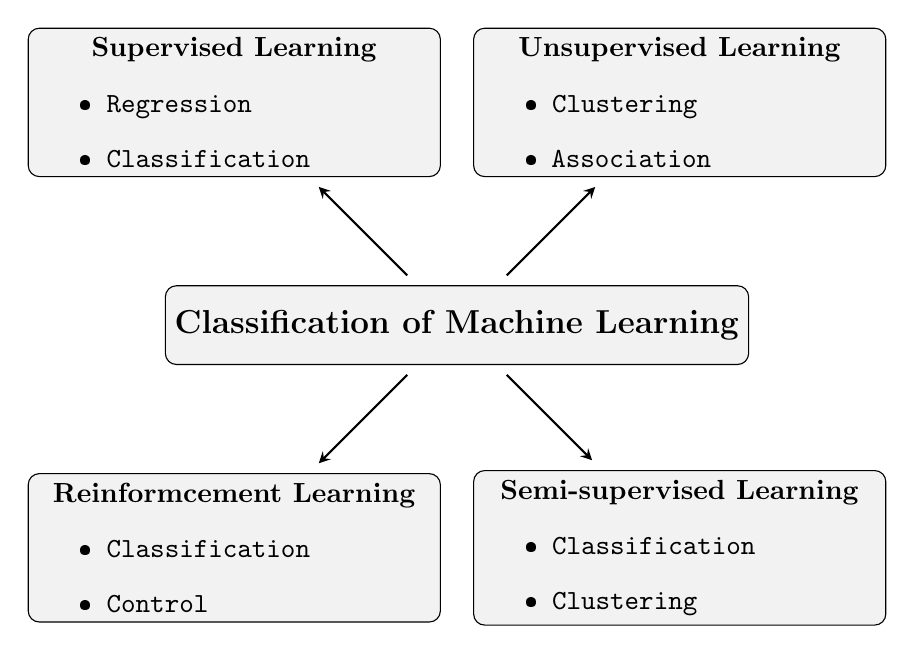
\begin{tikzpicture}[node distance=4cm]
		\node[box] (ml) {\large{\textbf{Classification of Machine Learning}}};
		\node[box, above left of = ml] (supervised) {
			\begin{minipage}{5cm}
				\centering\textbf{Supervised Learning}
				\begin{itemize}
					\item \texttt{Regression}
					\item \texttt{Classification}
				\end{itemize}
			\end{minipage}
		};
		\node[box, above right of = ml] (unsupervised) {
			\begin{minipage}{5cm}
				\centering\textbf{Unsupervised Learning}
				\begin{itemize}
					\item \texttt{Clustering}
					\item \texttt{Association}
				\end{itemize}
			\end{minipage}
		};
		\node[box,  below right of = ml] (semisupervised) {
			\begin{minipage}{5cm}
				\centering\textbf{Semi-supervised Learning}
				\begin{itemize}
					\item \texttt{Classification}
					\item \texttt{Clustering}
				\end{itemize}
			\end{minipage}
		};

		\node[box, below left of = ml] (reinforcement) {
			\begin{minipage}{5cm}
				\centering\textbf{Reinformcement Learning}
				\begin{itemize}
					\item \texttt{Classification}
					\item \texttt{Control}
				\end{itemize}
			\end{minipage}
		};
		\draw[arrow, shorten >= 5pt, shorten <= 5pt] (ml) -- (supervised);
		\draw[arrow, shorten >= 5pt, shorten <= 5pt] (ml) -- (unsupervised);
		\draw[arrow, shorten >= 5pt, shorten <= 5pt] (ml) -- (semisupervised);
		\draw[arrow, shorten >= 5pt, shorten <= 5pt] (ml) -- (reinforcement);
	\end{tikzpicture}
	\caption[Classification of Machine Learning]{The field of \acrlong{ml} divided into subfields by the characteristics of the underlying learning process. Also indicates the learning problems that are typically tried to be solved by utilising the respective learning process.}
	\label{fig:mlClassification}
\end{figure}

\subsubsection{Supervised Learning}
In supervised learning, the learning machine is provided with input data and the output that is expected for the given input. In the classical case of spam filtering, the input can be a collection of emails and the expected output is a label attached to each email that either classifies it as spam or as non-spam. The learning machine is then fed all e-mails as input data and learns to recognise which information in the input is important to claculate the correct classification. As the system knows the correct answer for each training input, it can process an email, predict wether it's spam or not, and then use the known answer to change its weights in a way that will make it more likely to lead to a correct prediction and less likely to lead to a false prediction the next time it is presented with a similar input.

\subsubsection{Unsupervised Learning}
Detecting patterns and structuring data is where unsupervised learning comes into play. Learners of this type don't need to be provided with an expected output while being trained. A scenario for the application of unsupervised learning is the problem of dividing a customer base into subgroups in order to treat every subgroup according to their specific needs. The employe might help the machine learning system by providing the number of subgroups he wants the system to generate. Most importantly however, he does not have to know the correct subgroup for the customers in the training data in order to solve this problem. The algorithms that tackle these learning problems are designed so that they can find structure in the data they are given and then also put new data in the best place given the current knowledge of the inherent structure in the overall dataset.

\subsubsection{Semi-Supervised Learning}

\subsubsection{Reinforcement Learning}

\subsection{Artificial Neural Networks}

An \gls{ann} - often just referred to as \gls{nn} - is a data processing concept that is inspired by biological neurons and their interconnectivity. As figures \ref{fig:2layeredANN} and \ref{fig:3layeredANN} show the artificial neurons (also called \textit{nodes}) in an \gls{ann} are grouped in \textit{layers}. There are three important types of layers: The \textit{input layer}\footnote{Note that the input layer is not counted towards the total number of layers in an \gls{ann}.}, the \textit{output layer} and an arbitrary number of \textit{hidden layers} in between the input and output layer. Similar to neurons in human brains, nodes of different layers can be connected. In \glspl{ann}, the nodes exchange signals in the form of numbers. Each node outputs a number that is computed by applying a non-linear function to its inputs. The output signal can then be a new input for other nodes or it can be part of the result returned by the output layer. The conncetions between nodes are also known as \textit{edges} and typically carry a weight. In the case of \glspl{ann}, the training process that is typical for all machine learning systems is the adjustment of these connection weights. The weights and other variables of the \gls{ann} are grouped under the term \textit{parameters}. Zusammengefasst transformiert ein \gls{ann} einen Inputvektor durch eine Reihe nicht-linearer Funktionen in einen Outputvekor, wobei sowohl die Berechnung des Outputs als auch der Trainingsprozess durch die spezifische Struktur des \gls{ann} und seine Parameter charakterisiert werden.

%TODO: Maybe introduce a view typical ANN architectures like feed forward, convolutional, recurring, etc.

\subsection{Deep Learning}

\Gls{dl} ist ein Teilbereich des Maschinellen Lernens. Charakteristisch für Deep Learning ist die Nutzung von \glspl{ann} mit vielen hidden layers. Je mehr hidden layers ein Netzwerk hat, desto tiefer ist es. Je tiefer ein Netzwerk ist und je mehr Nodes das Netzwerk pro Layer hat, desto komplexer sind die Berechnungen, die das \gls{ann} erfolgreich ausführen kann~\cite{dlBookGoodf}. Mit der wachsender Anzahl von Layern und Nodes wächst auch die Anzahl der Parameter. Ihre große Anzahl ist der Grund dafür, dass Deep Learning im Vergleich zu anderen Teildisziplinen des Maschinellen Lernens sehr große Datenmenge benötigt, um adäquate Ergebnisse zu liefern. Netzwerke dieser Gattung haben die Fähigkeit außerordentlich komplexer Berechnungen auf Kosten eines ressourcenaufwändigen Trainingsprozesses erhalten.

\begin{multicols}{2} % defines an environment with two columns
	\begin{figure}[H] % [H] for EXACTLY HERE
		\centering
		\includegraphics[height=3cm]{figures/ann1.jpeg}
		\caption[2-Layered ANN]{2-layered \gls{ann}. It is called fully connected as every node from the previous layer is connected to every node in the next layer. \\
			\tiny{Source:~\cite{annGraphics}}}
		\label{fig:2layeredANN} % labels always have to be placed after the caption
	\end{figure}
	
	\columnbreak    % start next column
	
	\begin{figure}[H] % [H] for EXACTLY HERE
		\centering
		\includegraphics[height=3cm]{figures/ann2.jpeg}
		\caption[3-Layered ANN]{3-layered \gls{ann}. In \glspl{ann}, nodes in one layer are connected to nodes in other layers but not to other nodes in the same layer. \\
			\tiny{Source:~\cite{annGraphics}}}
		\label{fig:3layeredANN} % labels always have to be placed after the caption
	\end{figure}
\end{multicols}

\section{A Core Task of Computer Vision: Object Detection}

\subsection{How Object Detection Differs From Related Tasks}

The field of computer vision umspannt eine Vielzahl unterschiedlicher Problemstellung und eine noch größere Anzahl möglicher Lösungsansätze. Im Folgenden wird die Objekterkennung als typische Aufgabenstellung im Computer Vision Kontext von den ihr von der Zielsetzung am nächsten stehenden Aufgabenstellungen abgegrenzt.

\begin{figure}[H] % [H] for HERE
	\centering
	\includegraphics[width=\textwidth]{figures/detection_related_tasks.png}
	\caption[Typical Computer Vision Tasks]{Object detection differs conceptually from other related computer vision tasks with regard to spatial information, the concept of objects and the number of detections in a given scene.\\
		\tiny{Source:~\cite{cvTasks}}}
	\label{fig:cvTasks} % labels always have to be placed after the caption
\end{figure}

\subsubsection{semantic segmentation}
Bei der segmantic segmentation wird jedem Pixel eines Bildes eine Klasse zugeordnet. Es gibt allerdings keine Objekte. Dies führt dazu, dass bei mehreren Objekten der gleichen Klasse im Bild, alle zugehörigen Pixel das gleiche Klassenlabel erhalten und die unterschiedlichen Objekte nicht anhand des Ergebnisses der semantic segmentation differenziert werden können.

\subsubsection{image classification (potentially including localisation)}
Bei der image classification ist das Ergebnis der detection immer ein einzelnes Objekt beziehungsweise dessen Klasse. In selten Anwendungsvarianten wird für das eine erkannte Objekt auch eine bounding box ausgegeben - in der Regel verbindet man mit dem task der classification allerdings keinen spatial extent.

\subsubsection{object detection}
Die Objekterkennung befasst sich mit der Identifizierung einer beliebigen Anzahl von Objekten innerhalb eines Bildes. Für jedes Objekt wird dabei ein Klassenlabel sowie seine Position in Form der Koordinaten eines das Objekt umspannenden Rechteckes ausgegeben. Wichtig hierbei ist, dass wie in Abbildung \ref{fig:cvTasks} erkennbar ist, auch mehrere Objekte der gleichen Klasse erkannt werden können. Die verschiedenen Objekte der gleichen Klasse sind dabei im Gegensatz zum vorherigen task der semenatic segmentation unterscheidbar.

\subsubsection{instance segmentation}
Die instance segmentation erfüllt im wesentlichen eine besser Variante der object detection. Es werden wieder mehrere Objekte verschiedener Klassen erkannt und die Positionen der Klassen mit ausgegeben. Dabei sind die Positionen allerdings nicht durch bounding boxes wie bei der object detection markiert, sondern jeder zu einem Objekt gehörende Pixel erhält ein Label dieses Objekts. Die Objekte werden daher noch schärfer von den Bildbereichen getrennt, die kein Objekt beinhalten und im Gegensatz zur semantic segmentation bleiben einzelne Objekte der gleichen Klasse unterscheidbar.


%\section{Computer Vision on Mobile Devices}

\subsection{Architectures}



\subsubsection{R-CNN}

2014
\cite{rcnnIntro}



%Heute Spielarten wie Fast R-CNN, Faster R-CNN, Mask R-CNN

\subsubsection{MobileNet}

2017

%In der Implementierung verwendet

\subsubsection{RetinaNet}

2018


\subsubsection{CenterNet}

2019

\subsubsection{EfficientDet}

2019

%YOLO
%ShuffleNet 2018
%FBNet 2019

\subsection{MobileNetSSDv2: A Single Shot MultiBox Detector}

\subsubsection{Introduction to XYZ Networks}


\subsubsection{Some Deep}
\subsubsection{Dive Into}
\subsubsection{Object Detection}
\subsubsection{Theory Fun}

\chapter{App Development}

\section{Previous State of the Application}

\subsection{Use Cases}

\subsection{Notable Design Decisions}

\section{Development Goals}

\subsection{Migration From Java to Kotlin}

\subsection{New Functionality: Object Detection}

\section{Implementing Object Detection Based on the TensorFlow Lite Framework}

\subsection{Some Deep}
\subsection{Dive Into}
\subsection{Object Detection}
\subsection{Implementation Fun}

\subsection{Next steps in the development of TUM-Lens}

% Potential Contets: Design and architecture choices, reused patterns from exisiting application, improvements to exisiting code

\chapter{Results}

\section{Performance}

\section{Accuracy}

\section{Possible Applications} % Can also be named "Future Work" depending on the contents of this section

Die Anwendungsbereiche von Computer Vision sind zahlreich. Zu den regelmäßigen Aufgaben im Bereich 

Organisation von Fotos auf dem Smartphone, ohne dass diese an die Server von Apple, \& Google Co geschickt werden müssen (Gruppieren von Fotos, die zu einem Urlaub gehören, Gesichtserkennung, Objekterkennung)

Autonome Autos werden unahängig von einer Verbindung zum Internet (5G, shared medium, bleibt das Auto im Tunnel dann stehen?)




% -------------------------------------------------------------------------------
% ----------------------------------- APPENDIX --------------------------------
% -------------------------------------------------------------------------------

\appendix

\chapter{Screenshots of the Application}

\chapter{Tips With Greetings From the Chair}
\label{sec:tips}       % labels can be put almost anywhere and can be referencef from anywhere.
Here are tips along the way:

\section{Tips}
\subsection{How to Describe}
% optional: set the spacing between columns
\setlength{\columnsep}{30 pt}
When listing several points you have three basic options:
\begin{multicols}{3}
	\begin{itemize}
		\item itemize
		\item enumerate
		\item description
	\end{itemize}
	
	\vfill\null
	\columnbreak
	
	\begin{enumerate}
		\item itemize
		\item enumerate
		\item description
	\end{enumerate}
	
	\vfill\null
	\columnbreak
	
	\begin{description}
		\item[itemize] short, unordered
		\item[enumerate] short ordered
		\item[description] listing of descriptions. Also nice for longer ones.
	\end{description}
	
\end{multicols}


\subsection{How to Quote}

\begin{quote}
	"This is a quote!"
\end{quote}

\begin{itemize}
	\item Citations to a source can be made like this \verb|\cite{gratl17task}| =~\cite{gratl17task}
	\subitem Always join text and the citation with a non-breaking space: \verb|text~\cite{foo}|.
	\item Referencing Sections, Figures, Tables, Formulas: \verb|\autoref{sec:tips}| = \autoref{sec:tips}.
	\item Footnotes for url or further notes: \verb|\footnote{\url{https://www.top500.org}}| = \footnote{\url{https://www.top500.org}}
\end{itemize}

\subsection{How to Math}

Use the align environment for equations especially if you want to align them somehow.

\begin{align}
	1 + 1 &\ne 3\\
	\left(\dfrac{10}{1}\right) - 9 &= 1
\end{align}

% if you need a pagebreak because figure placement is broken:
\clearpage

\section{Environments}

\subsection{How to Figure}

Anything can also be put in multiple columns.

\begin{multicols}{2} % defines an environment with two columns
	\begin{figure}[H] % [H] for HERE
		\centering
		\includegraphics[width=.9\columnwidth]{figures/scenario_clip_rot.png}
		\caption[Example Figure]{Some Caption. Always also include a source if it wasn't created by you!\\
			\tiny{Source:~\cite{gratl17task}}}
		\label{fig:exampleLabel1} % labels always have to be placed after the caption
	\end{figure}
	
	\columnbreak    % start next column
	
	\begin{figure}[H]
		\centering
		\begin{tikzpicture}
			\node[anchor=south west,inner sep=0] (image) at (0,0) {\includegraphics[width=.9\columnwidth]{figures/scenario_clip_rot.png}};
			\begin{scope}[x={(image.south east)},y={(image.north west)}]
				\draw[red, thin,rounded corners] (.42,.42) rectangle (.58,.6);
			\end{scope}
		\end{tikzpicture}
		\caption[Figure with tikz]{Figures can be drawn on or completely generated with tikz.}
		\label{fig:exampleLabel2}
	\end{figure}
\end{multicols}

\paragraph{Subfigures}
If grouping of several pictures seems reasonable, think about using subfigures. This often comes in handy with plots.

\begin{figure}[H]
	\centering
	\begin{subfigure}[b]{0.33\textwidth}
		\includegraphics[width=\textwidth]{example-image-a}
		\caption{example-image-a}
		\label{fig:example-image-a}
	\end{subfigure}
	\begin{subfigure}[b]{0.33\textwidth}
		\includegraphics[width=\textwidth]{example-image-b}
		\caption{example-image-b}
		\label{fig:example-image-b}
	\end{subfigure}
	\begin{subfigure}[b]{0.33\textwidth}
		\includegraphics[width=\textwidth]{example-image-c}
		\caption{example-image-c}
		\label{fig:example-image-c}
	\end{subfigure}
	\caption{One caption to describe them all.}
\end{figure}

\subsection{How to Algorithm}

\begin{figure}
	\begin{algorithm}[H]
		
		% Define custom keywords
		\SetKwFunction{KwNot}{not}
		% Define custom Functions
		\SetKwFunction{Fissorted}{is\_sorted}
		\SetKwFunction{Fbogosort}{bogosort}
		\SetKwFunction{Fshuffle}{shuffle}
		\SetKwProg{Fn}{Function}{:}{}
		\KwIn{\tabto{2cm}data array}
		\KwOut{\tabto{2cm} data sorted}
		\BlankLine
		
		\tcp{Checks if array is sorted}
		\Fn{\Fissorted{data}}{
			\For{i $\leftarrow$ 0 \KwTo data.size() - 1}{
				\label{algo:for}            % labels can also be put in the algorithm
				\If{data[i] $>$ data[i+1]}{
					\Return false
				}
			}
			\Return true
		}
		
		\tcp{actual algorithm}
		\Fn{\Fbogosort{data}}{
			\While{\KwNot \Fissorted{data}}{
				random.\Fshuffle{data}
			}
		}
		
		\caption[Bogosort]{Bogosort}
		\label{algo:example}
	\end{algorithm}
	\caption{some description what is happening}
\end{figure}

\clearpage

\subsection{How to Code}
\begin{lstlisting}[style=eclipse-cpp, caption=General form of a typical runner() function., label=code:runner]
	void runner(int type, void *data){
		switch(type)
		case taskType1:
		// do stuff using data
		case taskType2:
		// do other stuff using data
	}
\end{lstlisting}

\subsection{How to Table}
\begin{table}[H]
	\begin{tabularx}{\columnwidth}{L | C | R}
		\hline
		\hline
		bla left & bla centered\newline over two lines &  bla right\\
		\hline
		bla left & bla centered & \multirow[c]{2}{\hsize}{cell spanning two rows} \\
		\cline{1-2}
		\multicolumn{2}{c|}{cell spanning two columns} & \\
	\end{tabularx}
	\caption[Some Table]{Fancy table that can contain line breaks and extended cells.}
	\label{tab:example}
\end{table}

%TODO: Insert screenshots. Potentially even with the respective old version of a screen to see the development.

\listoffigures

\listoftables

\printbibliography

\printglossary[type=acronym,nonumberlist]

\printglossary[type=main,nonumberlist]

\end{document}
